\documentclass[12pt, landscape]{article}
\usepackage[scaled=0.92]{helvet}
\usepackage{multicol}
\usepackage{calc}
\usepackage{ifthen}
\usepackage[landscape]{geometry}
%\usepackage{hyperref}

\usepackage{newtxtext} 

%for strikeout
\usepackage{ulem}

%For editing parbox
\usepackage[table]{xcolor}
%For editing itemise margins, reduce iterm separaion and list separation
\usepackage{enumitem}
% For math
\usepackage{amsmath,amsthm,amsfonts,amssymb}

%For pictures / figures
\usepackage{color,graphicx,overpic}
\graphicspath{ {./images/} }

%\usepackage{newtxtext} 
%\usepackage{amssymb}
%\usepackage[table]{xcolor}
%\usepackage{vwcol}
%\usepackage{tikz}
%\usepackage{wrapfig}
%\usepackage{makecell}

\pdfinfo{
  /Title (IS2238.pdf)
  /Creator (Ger Teck)
  /Author (Ger Teck)
  /Subject ()
  /Keywords (tex)}

%% Margins for PAPER

% This sets page margins to .5 inch if using letter paper, and to 1cm
% if using A4 paper. (This probably isn't strictly necessary.)
% If using another size paper, use default 1cm margins.
\ifthenelse{\lengthtest { \paperwidth = 11in}}
	{ \geometry{top=.5in,left=.5in,right=.5in,bottom=.5in} }
	{\ifthenelse{ \lengthtest{ \paperwidth = 297mm}}
		{\geometry{top=1cm,left=1cm,right=1cm,bottom=1cm} }
		{\geometry{top=1cm,left=1cm,right=1cm,bottom=1cm} }
	}

% Turn off header and footer
\pagestyle{empty}

% for tight centres (less spacing)
\newenvironment{tightcenter}{%
  \setlength\topsep{0pt}
  \setlength\parskip{0pt}
  \begin{center}
}{%
  \end{center}
}

% Redefine section commands to use less space
\makeatletter
\renewcommand{\section}{\@startsection{section}{1}{0mm}%
                                {-1ex plus -.5ex minus -.2ex}%
                                {0.5ex plus .2ex}%x
                                {\normalfont\large\bfseries}}
\renewcommand{\subsection}{\@startsection{subsection}{2}{0mm}%
                                {-1explus -.5ex minus -.2ex}%
                                {0.5ex plus .2ex}%
                                {\normalfont\normalsize\bfseries}}
\renewcommand{\subsubsection}{\@startsection{subsubsection}{3}{0mm}%
                                {-1ex plus -.5ex minus -.2ex}%
                                {1ex plus .2ex}%
                                {\normalfont\small\bfseries}}
% change font
%\renewcommand{\familydefault}{\sfdefault}
%\renewcommand\rmdefault{\sfdefault}
\makeatother

% Define BibTeX command
\def\BibTeX{{\rm B\kern-.05em{\sc i\kern-.025em b}\kern-.08em
    T\kern-.1667em\lower.7ex\hbox{E}\kern-.125emX}}

% Don't print section numbers
\setcounter{secnumdepth}{0}

\setlength{\parindent}{0pt}
\setlength{\parskip}{0pt plus 0.5ex}

%% this changes all items (enumerate and itemize, reduce margins)
\setlength{\leftmargini}{0.5cm}
\setlength{\leftmarginii}{0.5cm}
\setlist[itemize,1]{leftmargin=2mm,labelindent=1mm,labelsep=1mm, itemsep = 1mm}
\setlist[itemize,2]{leftmargin=4mm,labelindent=1mm,labelsep=1mm, itemsep = 1mm}
\itemsep = 2mm
%\setlist{nosep}

% -------------------------------------------------------------------------------

% START OF DOCUMENT HERE

\begin{document}
\raggedright
\footnotesize
\begin{multicols*}{3}

% multicol parameters
% These lengths are set only within the two main columns
\setlength{\columnseprule}{0pt}
\setlength{\premulticols}{1pt}
\setlength{\postmulticols}{1pt}
\setlength{\multicolsep}{2pt}
\setlength{\columnsep}{2pt}

%% DOCUMENT NAME HERE
\begin{center}
     \Large{\textbf{IS2238 Economics of IT \& AI}} \\
\end{center}

% TABLE PACKAGE 
 \begin{center}
    \fbox{%
        \parbox{0.8\linewidth}{\centering \textcolor{black}{
            \\ \normalsize{AY22/23 Sem 2}}
            \\ {\footnotesize github.com/gerteck}
        }%
    }
 \end{center}

\section{1. Overview of Economics of IT}

\begin{itemize}
	\item \textbf{IT/AI are changing our lives, businesses, and economy.} Economics can provide a lens through which we can better understand this new economy and phenomena in a more systematic manner.
	\item High speed change in today’s digital age. (Digital revolution). Cause of change is computer \& comunications, technology such as integreted circuits, data speed and laptop capacity which have increased by many times. $\rightarrow$ Increase in employee productivity.
	\item \textbf{Moore’s Law:} observation that the numer of transistors on a microchip doubles every 18-24 months (exponential growth). Advancement has slowed down since 2010s.
	\item \textbf{Why does IT matter for today's economy?}: IT capital investment by companies has grown steadily over the years from 1980s to 2010. Market capitalization has seen most large companies being tech related or heavily invested in IT.
	\item \textbf{Economics:} Allows for systematic understanding of new phenomena. This provides a lens through which we can better understand how things work, design clever solutions and create the conditions in which we can all flourish. We do this through economic theory, methods, analytical methods, empricial modelling.
	\item \textbf{Evaluating IT investment and its impact:} IT investments by firms do not necessarily lead to better outcomes nor better lives. Question has important policy and managerial implications. There are many variables to consider, such as obsolescence of old technologies, cost of learning, infrastructures, poor IT management, underutilization. Companies need to throughly understand the role and impact of IT on their business models and the exact use if implemented.
	\item \textbf{IT Productivity Paradox}: Economist Robert Solow: a Nobel Prize laureate, famously said in 1987, “You can see the computer age everywhere but in the productivity statistics”. It was largely resolved by an economics analysis done by MIT professor Erik Brynjolfsson and his colleagues in in the mid-1990s. Cobb–Douglas production function.
\end{itemize}

\subsection{Cobb-Douglas Production Function} 
models the relationship between production output and production inputs (factors).
\centerline{$Y = AL^\beta K^\alpha$}
\\ Y: Total Production, L: Labor Input,
\\ K: Capital Input, A: Total Factor Productivity,
\\ $\alpha$ and $\beta$: output elasticities of capital and labour.
~\\ ~\\
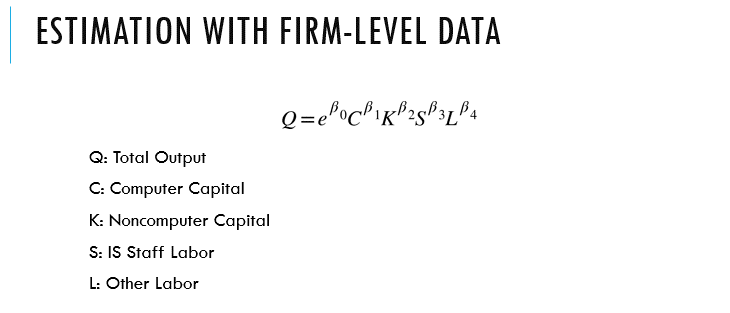
\includegraphics[width=\linewidth]{firmLevelData}

~\\

\textbf{Insights:} Brynjolfsson and Hitt (Management Science, 1996)
\begin{itemize}
\item An additional dollar of computer capital stock is associated with an increase in output of 81 cents per year on the margin An additional dollar spent was associated with a marginal increase in output of \$2.62
\end{itemize}

\vfill\null
\columnbreak

\section{2. Digital Economy and New IT}
\subsection{McKinsey View on 'New' IT}
\begin{itemize}
\item Numerous industries being `reimagined' through IT: To prevent a competitor from re-imagining your product as discontinued or re-imagining your company into liquidation, IT could well be an essential consideration in strategy formulation and execution, and a key area for investment.
\item `Old IT': Addressed labor automation, individual worker productivity, and non-human scale computing;
\item `New IT': Focus on digital products and services, team productivity, and business model transformation.
\item Benefits from old IT have reached a point of diminishing returns; new IT can be a source of competitive differentiation and dramatic wealth creation.
\item \textbf{Business Model Transformation} as a major use of IT, five major levers: Production and operations optimization, Eliminating intermediaries (bypassing middleman), New Monetization models (Amazon Web Services, SaaS etc.), Shaping customer preferences (leveraging big data), Transforming underserved markets (Long Tail phenomenon).
\end{itemize}

\subsection{Traditional Supply Chain Issues}
\begin{itemize}
\item Lack of Coordination between stages in the supply chain where objectives of different stages conflict or information moving between stages is distorted.
\item \textbf{Bullwhip Effect:} Fluctuations in order increases as they move up the supply chain from retailers to wholesalers to manufacturers to suppliers. Distorted demand information, where different stages have different estimates of what demand looks like, amplified variation in demand. Higher safety inventory usually required.
\item Information Processing Obstacles: Forecasting demand based on orders, not customer demand. Lack of information sharing. To overcome tradeoff, we trade responsiveness for cost and vice versa.
\end{itemize}

\subsection{Just-In-Time Production Methods}
\begin{itemize}
\item Tesla Motors has been using Just-In-Time (JIT) production methods to keep costs low since its founding in 2003. (JIT Benefits + Challenges) Tesla is experimenting with lean manufacturing principles in its production processes.
\item JIT is a production strategy that seeks to minimize waste and maximize efficiency by only producing what is needed, when it is needed. This approach requires close coordination between all parts of the production process, from suppliers to assembly line workers.
\item There are some chalenges associated with JIT, such as the need for tight coordination and the potential for disruptions to the production process. However, Tesla has shown that JIT can be an effective production strategy for a high-tech manufacturing company.
\end{itemize}

\subsection{Digital Economy}
\begin{itemize}
\item \textbf{A Digital Economy} takes advantage of the latest technology to digitalise processes and drive business growth. With digital economy, most of economic activities such as production, distribution, and consumption of goods and services are digitalized.
\item Digital technologies reduce the cost of storage, computation, and transmission of data. Therefore, digital economics explores how standard economic models change as certain costs fall substantially and perhaps approach zero.
\item \textbf{IT Capital Investment:} IT Capital Investment by companies has been increasing (in proportion and amount) over the years. IT automate many steps in business processes that were formerly performed manually. IT can enable new innovative business processes by collecting, processing, distributing information in a more efficient and effective way. (e.g., JIT, cross-docking) IT can transform the way the business works and drive new business models.
\end{itemize}
\subsubsection{Production and Economics of Production: Cost Curves}
\begin{itemize}
\item \textbf{Simple Economics of Production:}
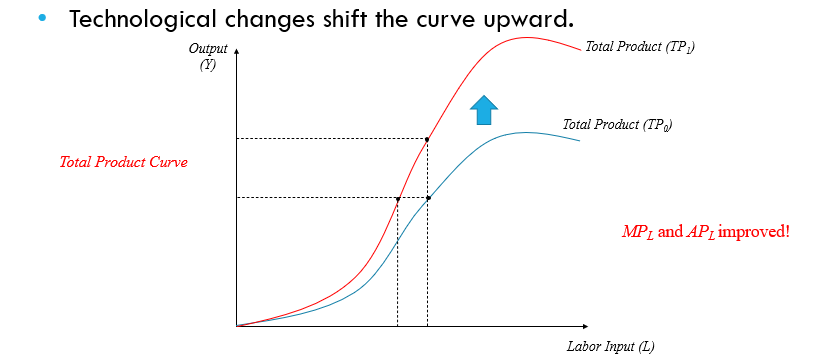
\includegraphics[width=0.7\linewidth]{technologicalChange}
\item \textbf{Economics of Digital Goods:} High fixed costs to produce the first unit, dominated by sunk cost: very high. Marginal production (reproduction) cost : very low. Hence, extensive economies of scale. Can be delivered via the Internet; little distribution cost.
\item DD and SS curve shifts as an impact of technological advances: Demand depends on the presence of substitutes or complements, Supply generally increases production cost drops.
\end{itemize}

\subsection{Disadvantages of Digital Economy}
\begin{itemize}
\item Digital divide: Generally refers to the gap between those who use or have access to telecommunications and information technologies including hardware, internet access, and literacy in using both effectively and those who do not.
\item Cybercrime and Privacy Breaches, Bad ideas spread quickly (e.g., fake news, racism, etc.), Pervasive Advertisement exposure (due to New business model), More monopolistic players (e.g., Google), Addictive nature of technology (Mental health and well-being concerns)
\end{itemize}

\textbf{Summary (of digital technology on businesses)}
\begin{itemize}
\item Digital technology enables economic activities such as production, distribution, and consumption of goods and services are conducted in a more efficient manner.
\item On top of that, digital innovation may lead to a fundamental change through a new economic rule, enhanced collaboration, and innovative business models.
\item However, some other challenges may also arise because of digital technologies
\end{itemize}

\vfill\null
\columnbreak

\section{3. Market Structure}
\begin{itemize}
\item \textbf{Market Power / Dominance} is the ability of a firm or group of firms within a market to profitably charge prices above the competitive level for a sustained period of time. Due to anti consumer and anti competitive issues, huge market power always reduces the economic wealth of society in many ways. (Sherman Antitrust Act US, M\&A regulation, price regulation.)
\item Surge in IT investment by firms from 1995: Internet and enterprise IT accelerated competition within traditional industries. Processes were digitalized through enterprise IT systems. Innovators dominate the market with better ways of doing things. Rivals recapture market shares by roling out further process innovations. Results in increased concentration, turbulence and performance spread.
\subsection{Market Structures (basic economics)}
\item \textbf{Perfect Competition}: Many buyers and sellers with small size, Homogeneous product (little differentiation), Perfect information for buyers and sellers, No transaction/switching costs in market, Free market entry and exit, Equal access to technologies, Company as a price taker. Equilibrium = Normal Profits
\item \textbf{Monopolistic Power}: A monopoly is a company that has "monopoly power" in the market for a particular good or service. The existence of a monopoly relies on the nature of its business. It is often one that displays one or several of the following qualities: Needs to operate under large economies of scale, Requires huge capital, No substitute, Government mandate ensuring its sole existence, Technological superiority and control resources. Disadvantages of a monopoly: Price fixing, declining product quality, loss of innovation, inflation.
\\ Arguments for a `Creative Monopoly': Some advantages of monopoly may include: Economies of scale, Stability of prices, R\&D spending.
\item \textbf{Oligopoly:}: An oligopoly consists of a select few companies that combined exert significant influence over a market or sector. Firms in this case either compete with another to collaborate together (collusion). They use their market influence to set the prices and in turn maximize their profits. Therefore, the consumers become the price takers. In an oligopoly, there are various barriers to entry in the market, and new firms find it difficult to establish themselves. Most countries have laws outlawing such anti-competitive behaviors. Think FAANG or MANGA.
\end{itemize}


\subsection{Porter's Five Forces Framework}
Five forces that determine the competitive intensity and therefore attractiveness of a market.
\begin{itemize}
\item A useful tool (i) to understand the attractiveness of an industry and (ii) to systematically analyze the external environment surrounding a firm. Overall industry attractiveness does not imply that every firm in the industry will return the same profitability. Competitive advantage of a firm is achieved by enhancing a firm’s ability to combat the 5 forces.
\item \textbf{Force 1: Bargining Power of Supplier}: Supplier power is high when there is domination of supply by a few companies. (Examples: Crude Oil Suppliers (OPEC)), product is unique or at least differentiated, has built up switching costs (Examples: Database (Oracle), MS Windows, Cell phone services), provides benefits through geographic proximity to its customers. ( Examples: Convenient stores), poses a definite threat to forward integrate into its customers’ business. (Examples: Movie studios that also own a chain of theatres).
\item \textbf{Force 2: Bargining Power of Buyer/Consumer}: Buyer’s bargaining power is high when it has large, concentrated buying power that enables it to gain volume discounts and/or special terms or services (Examples: organizational buyers like Wal-Mart, Costco, Safeway), what it is buying is standard or undifferentiated and there are multiple alternative sources, product is unimportant to the quality of the buyers’ products or services. (Examples: buyers of commodity type of products), has a strong potential to backward integration. (Examples: airline companies that also own aircraft maintenance and in-flight catering businesses).
\item \textbf{Force 3: Substitute Products or Services}: Substitutes: a product or service in another industry which can fulfill the same needs. Threat of substitute products or services is high when  Relative price performance of substitutes is high, Switching cost to new products is low, Buyer propensity to substitutes is large.
\item \textbf{Force 4: Threat of Potential New Entrants}: The threat of new entrants is high when it is easy for new competitors to enter a market, low when there are significant entry barriers to entering a market. Common sources of the entry barrier include: Regulation, Patents and proprietary knowledge, Economies of scale: Newcomer’s cost per product is higher, Capital requirement, Difficulty in brand switching, Difficulty in accessing distribution channel.
\item \textbf{Force 5: Rivalry among Existing Competitors}: Intra-industry rivalry is intense when Competitors are numerous or roughly equal in size and power, Industry growth is slow, precipitating fights for market share, and the product lacks differentiation or switching costs.
\end{itemize}

\subsection{Internet's Impact on Industries \& Forces}
\begin{itemize}
\item \textbf{Impact on Industries}: High Industry concentration, High Turbulence (the top-selling company one year may not dominate next year. Today’s \#10 company, for instance, might jump to \#1 the following year.) Large and Growing Performance Spread: Increasing spread in gross profit margin.
\item \textbf{Impact on Market Structures}: `Easier to become a monopoly in Digital Economy': Network Effects (“Winner takes all” phenomenon) (value of service depends on number of users), High switching cost, Economies of scale, High initial fixed cost and low marginal cost of production. Convergence of digital services (Blending of previously separate technologies, processes, and data to create new combinations of products, services, and experiences that reshape industry structures It is much easier to create new services by combining multiple services), AI \& Data analytics, Hard to regulate.
\item \textbf{Digital Business vs. Traditional Market:} Market definition is complicated by zero-pricing for the use of many digital platforms and the subsequent harvesting of consumer data. For many digital platforms, consumers forfeit their data (rather than money) in exchange for the services they receive (e.g., Google, YouTube, etc).
\item \textbf{Impact on Competitive Dynamic of each Force}:  Adds entry barriers to new entrances, enables foothold in rivalry among existing competitors, adds to switching cost reducing buyer power. (e.g. American Airlines (SABRE) Reservation system, Display bias, 80\% of reservation conducted on first page, Information over competitor, Co-host program with partner airlines bargining power, new business creation, enabled AA to expand busines scope into information business.)
~\\ ~\\
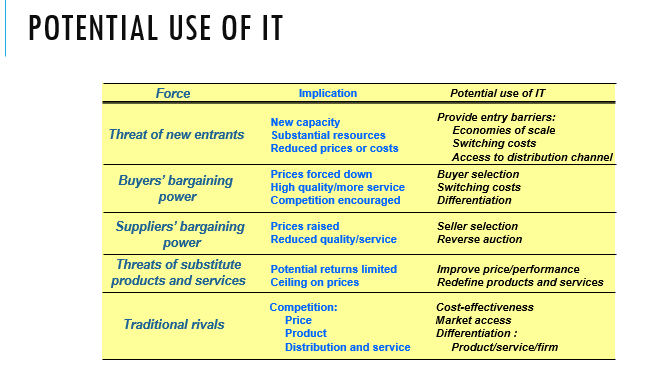
\includegraphics[width = \linewidth]{portersIT}
\\ ~\\
~\\ ~\\
\textbf{Internet's Impact on Five Forces:}
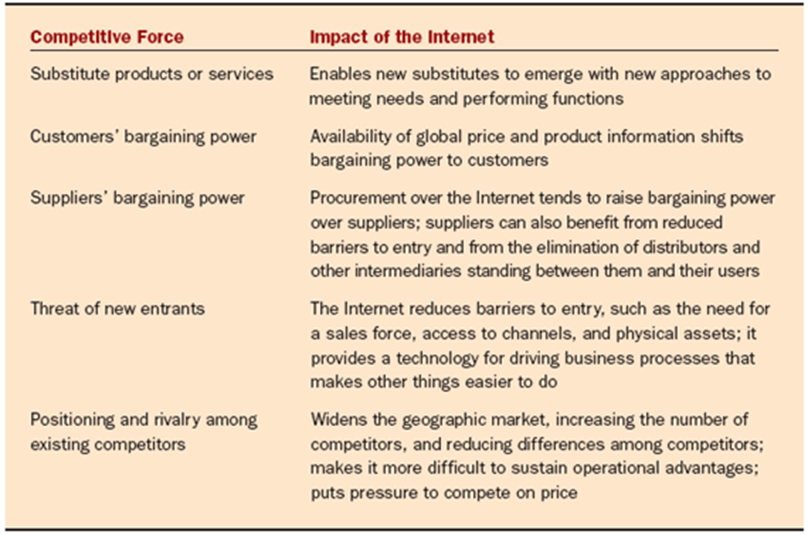
\includegraphics[width = \linewidth]{portersInternet}
\end{itemize}

\vfill\null
\columnbreak

\section{4. Pricing, Bundling and Subscription Model}
Pricing: (Most important determinant of consumption of goods/services. Aim for Profit maximizing price)
\subsection{Economic Value to Customer}
\begin{itemize}
\item \textbf{EVC:} Measure of how much value an individual customer, or customer segment, gets from using a company’s products or services: It includes both tangible and intangible benefits. Underlying economic theory: Customer will buy a certain product only if its utility to them outweights that of the closest alternatve (total satisfaction or benefit).
\centerline{\textbf{EVC = Reference Value $+$ Differentiation Value}}
\item Reference Value: Price of what customer views as the best substitute
\item Differentiation Value: Value of differentiating attributes over the best substitute.
\item \textbf{Sources of Customer Value}: Benefits or costs associated with availability, convenience, functionality, relationship, brand image. Example: Starbucks differentiation value through branding. 
\item  \textbf{Application of EVC: } EVC leads to maximum willingness to pay (WTP). EVC is determined by reference and differentiation value, consumer choices is determined by net value. Can derive demand curve based on understanding of customer value, and obtain profit maximizing price level.
\item \textbf{Developing Pricing Strategy}: In reality, customers are very different (heterogenous) in terms of taste and WTP. Must assess value customers place on product and WTP, through market research, customer contact, etc or qualitiative or quantitative methods.
\end{itemize}

\subsection{Price Discrimination}
Price Discrimination: Charging customers different prices for the same product. 
\begin{itemize}
\item \textbf{First degree (Perfect) price discrimination}: Individual pricing (personalized pricing): Becoming easier, but may face some controversies and resistance (Amazon price-testing program raises anger, cola vending machine price related to temperature, singer album price increase after death)
\item \textbf{Second degree price discrimination}: (versioning or menu pricing): Create different products for the purpose of price differentiation (Easily done for Software → Full features and value-subtracted to target different segments, e.g. math software pro vs student version, quicken software). Versioning: firm engages in differential pricing by offering different versions of a product, e.g. IBM spent additional money to insert a chip to slow down one of its printers → Marginal cost is incurred! However, for digital products, creation of different versions is so easy for digital goods/services! (because MC=0).
\item \textbf{Third degree price discrimination}: Group pricing based on segmentation, when a company charges a different price to different consumer groups. Firms try to generate sales by identifying different market segments, such as domestic and industrial users, with different price elasticities. (e.g. Student or Senior Price) Identifying such segments and implementation of differential prices have become much easier with digital technologies! Digital technologies including AI-based methods enable such price discrimination at more affordable costs
\end{itemize}

\subsubsection{Using Big Data to adopt Price Discrimination:}
3Vs: Volume, Velocity and Variety of Data.
\begin{itemize}
\item \textbf{Volume}: A large amount of data, which makes the conventional approaches and algorithms inefficient and less applicable.
\item \textbf{Velocity}: Real-time or nearly real-time information makes it possible for a company to be much more agile than its competitors.
\item \textbf{Variety}: Many sources, different data formats, highly unstructured (Messages, images, videos, readings from sensors, GPS signals from cell phones, etc)
\item These data help firms better understand customers and develop accurate and more effective pricing strategies. How? → Price discrimination
\\ ~\\ ~\\ ~\\
\item \textbf{Types of Data categorised via 3Vs}
~\\ ~\\
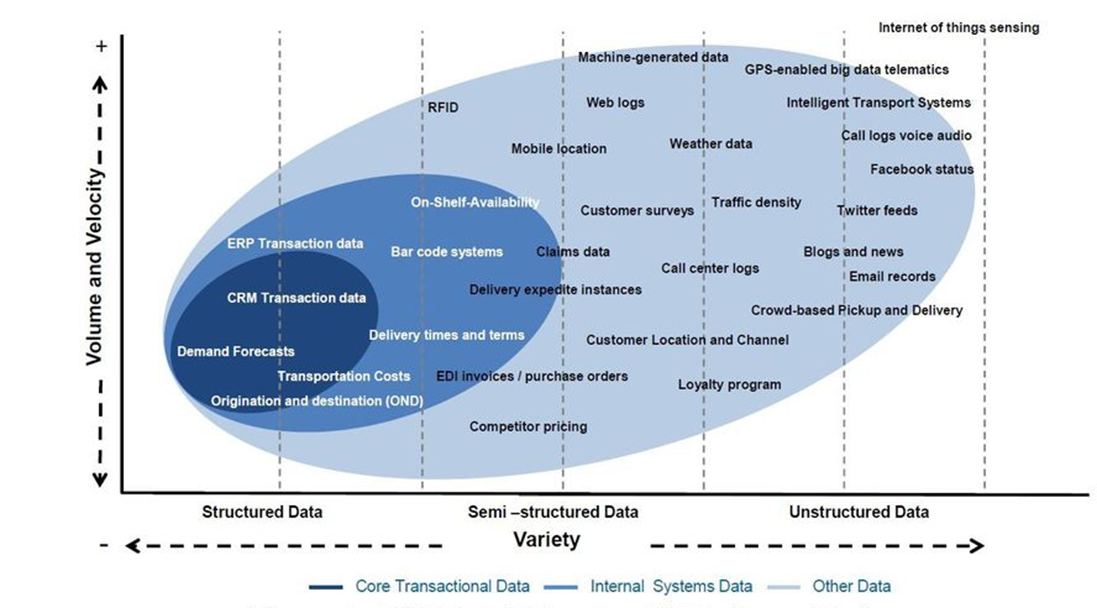
\includegraphics[width = \linewidth]{bigData3V}
\end{itemize}


\subsection{Capturing Consumer Information and using it with AI }
\begin{itemize}
\item \textbf{Marketing Funnel}: A series of stages to guide prospects through the customer journey. Crucially, what data do they need at each stage?
~\\ ~\\
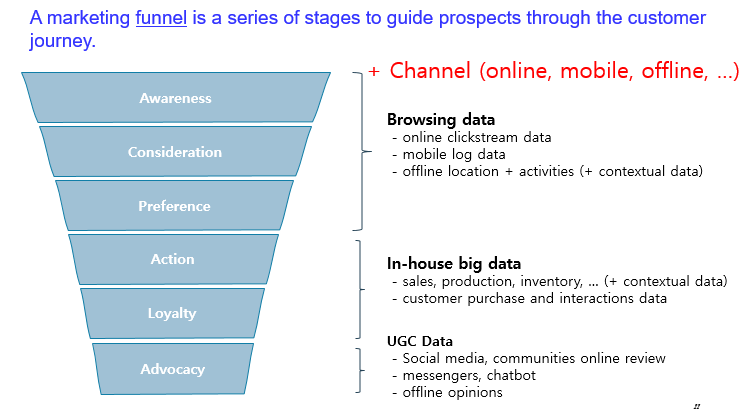
\includegraphics[width = \linewidth]{marketingFunnel}
\item \textbf{User Generated Content UGC}:UGC is at least as valuable as a source of customer needs for product development, likely more valuable, compared with conventional methods. Machine-learning methods improve efficiency of identifying customer needs from UGC (unique customer needs per unit of professional services cost). (See potential system architecture for identifying customer needs from UGC.) E.g. Study Timoshenko et al (2019): UGC captures vast majority of customer needs (97\%), opportunities for prodct improvement (92\%) and hidden opportunities (92\%)for oral-care products.
\end{itemize}

\subsection{Bundling: (Combining products and pricing)}
\begin{itemize}
\item Can be considered a form of (second degree) price discrimination, Discriminate by quantity and features. 
\item Bundling can be also easily done through digital technologies! (low menu cost, marginal cost, cost of implementation, etc)
\end{itemize}

\subsection{Subscription Model: (Type of PD and bundling)}
\begin{itemize}
\item Businesses may benefit because of predictable and constant revenue stream from subscribed individuals.
\item Many digital services are offering a subscription-based pricing.
\end{itemize}

\textbf{Summary}: Consumers are heterogenous, making different pricing strategies more effective. Digital technologies have enabled firms to extract more surplus from consumers because it is now easier to estimate their WTP and implement different pricing schemes for price discrimination (low marginal cost of production, lower menu cost, low cost of implementation).


\vfill\null
\columnbreak

\section{5. Network Effects }

\subsection{Externalities}
\begin{itemize}
\item \textbf{ An externality}: an indirect cost or benefit to an uninvolved third party that arises as an effect of another party's (or parties') activity. That is, an externality is an event the occurs as a byproduct of another event occurring. Can be positive or negative and can stem from either the production or consumption of a good or service.
\item Example: R\&D of a company can be a positive externality. R\&D increases the private profits of a company but also has the added benefit of increasing the general level of knowledge within a society. Pollution caused by commuting to work or a chemical spill caused by improperly stored waste are examples of negative externalities.
\end{itemize}
\subsection{Network Effects}
\begin{itemize}
\item\textbf{Network Effect} is the phenomenon by which the value or utility a user derives from a good or service depends on the number of users in general and user connection in particular, in the product/service network.
\item Network effects are typically positive (i.e., positive externalities), resulting in a given user deriving more value from a product as more users join the same network.
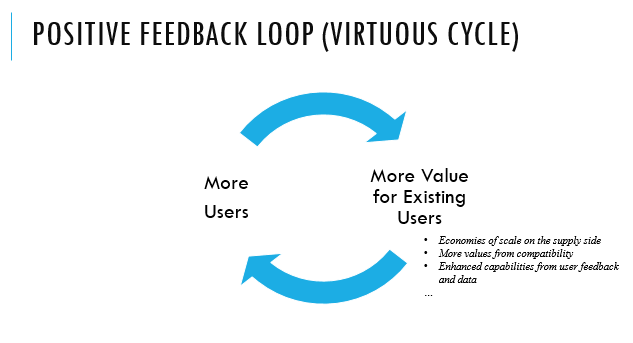
\includegraphics[width=\linewidth]{positiveFeedbackLoop}
\item Congestion is a negative network effect whereby too many users can slow a network down, reducing its utility and frustrating network members.
\item \textbf{Metcalfe's law} states that the value of a telecommunications network is proportional to the square of the number of connected users of the system. (1993) Assumes all nodes have equal benefits and are all connected, but many social networks don’t exactly match Metcalfe law because some new nodes don’t create connections with all existing nodes. Also, In social networks, new entrants that join later and have different interests and expertise may not create connections with existing users. This decreases benefit of each additional user, making the overall network less efficient if costs per users are fixed.
\end{itemize}
\subsection{Network Effects in Digital Economy}
\begin{itemize}
\item Network effects have become a defining property of the digital economy, since the business model of many digital services is based on matchmaking (e.g., Uber, Airbnb, Gig economy platforms) and mediation between users (e.g., YouTube, Facebook).
\item The positive feedback is not totally new but is a \textbf{more potent force} in the digital economy than ever before, often leading to a \textbf{winner-takes-all market}.
\item \textbf{AI and Positive Feedback (of usage)}: Good data can lead to a positive feedback loop with advanced decision recommendation and analytics today. It would be more critical in the age of AI. However, having good data for training of algorithms may be challenging in certain contexts.
\end{itemize}
\subsection{Impact of Network Effects on Pricing: Freemium Models}
\begin{itemize}
\item \textbf{Price Differently}: As a business grows due to the network effect, it often makes sense to increase prices as demand for the product grows. However, starting at a lower price (or in some cases, giving the product away for free, as mentioned above) and then increasing the price of the product as the network effect occurs will result in a larger user base.
\item \textbf{Freemium}: business model in which a company offers basic or limited features to users at no cost and then charges a premium for supplemental or advanced features. Freemium models are especially popular among software applications and internet-based businesses (partly because MC=0).
\end{itemize}
\subsection{Two-sided Network (Platforms) Effects}
\begin{itemize}
\item \textbf{Two-sided networks}: Products and services that bring together groups of users in two-sided networks are platforms. Examples: Operating Systems, B2B Exchanges, Online recruitment.
\item Platforms provide infrastructure and rules to facilitate the two groups’ transactions and can take many forms. When successful, the platforms catalyze a virtuous cycle; More demand from one side spurs more from the other. (e.g. Ebay)
\end{itemize}
\subsection{Effective Strategies \& Considerations in Presence of Two-Sided Network Effects}
In the e-commerce environments, you may have to deal with the two-sided network effects. It is tricky to manage platforms successfully
\begin{itemize}
\item \textbf{Disruptive Force}: Disrupting Existing Networks (Zoom vs Skype): Zoom is actually built on allowing “frictionless” communication between users the service is not meant to only work for those in its network, where zoom user can video call anyone by sending link, where recipient does not even need to have a Zoom account.
\item \textbf{Pricing}: Subsidize one user group (quality and price sensitive users) while charging the other a premium for access to the subsidized group (E.g., Adobe’s Acrobat PDF maker). Secure important users’ exclusive participation in your platform by providing incentives (E.g., government, LV in the airport).
\item \textbf{Coping with Winner-Takes-All Competition}: Decide whether the two-sided market you’re eyeing will eventually be served by a single platform. If yes, it is risky to fight for proprietary control (E.g., Video players, App Store).
\item \textbf{Consumer Protection and Legal Issues}: Examples: Counterfeit products on e-commerce websites, Legal responsibilities for platform “gig” workers, Consumer privacy and data breaches, can affect company stock prices.
\end{itemize}

\vfill\null
\columnbreak


\section{6. Lock-in and Switching Costs}
\textbf{Lock-In} is making customers dependent on them for products and services by making it hard to switch to a competitor without substantial costs.
\begin{itemize}
\item \textbf{Customers}: Reluctant to switch from existing choices, Costs of switching $>$ Gains from switching, Customers face lock in into current choices, Want to avoid lock-in as decisions made today which limit future options.
\item \textbf{Sellers}: Aim to lock in customers, Captive customers, who are reluctant to substitute one product or vendor due to high cost, which are the greatest asset, Use diverse strategies.
\item \textbf{Lock in} is a common strategy in IT industries. User base is key (first-mover advantage). Business flexibility is high. IT business create “Ecosystems” or “Platforms”. Example: substantial heterogeneity in switching costs across online broker site providers. Reduce switching is attributed and related to systems usage, system quality and personalisation.
\end{itemize}
\textbf{Switching Cost}: Switching costs are costs that a consumer incurs from switching brands, products services or suppliers. The higher the cost, the more likely an individual will be willing to lock in.
\begin{itemize}
\item Switching costs include financial costs (e.g. price, compensation, incentives) and non-financial costs, such as psychological, time and effort-based costs.
\item \textbf{Measuring Switching Costs}: Total switching costs $=$ Customer’s costs of stopping usage of firm A’s product $+$ Firm B’s cost. 
\item This is such that customer C switches from firm A to B. Subsidies or incentives may be used to induce switch. (e.g. side payments, compensation, gift cards.)
\item \textbf{EVC}: The Economic value to consumer. The cost of stopping purchase or usage of A’s product often lies in its competitive advantage
\end{itemize}
\subsection{Lock-in and Market Failure}
\begin{itemize}
\item \textbf{Technological lock in} is a form of economic path dependence whereby the market selects a technological standard. The market players get locked in or stuck with standard even though alternatives may be better. (E.g. QWERTY vs Dvorak keyboard). First user experience becomes de facto standard. 
\item Some economist argue that technological lock in on the free market leads to the potential of an inferior choices. Governments or mandatory industry boards may step in to correct the supposed market failure. (e.g. USB-C common charger to reduce e-waste of unused chargers.)
\end{itemize}
\subsection{Classification of Lock-in}
\begin{itemize}
\item \textbf{Types of lock-in} have become more prevalent with digital technologies: Contractual commitments, brand-specific training, information and databases, search costs, loyalty programmes.
\begin{itemize}
\item \textbf{Brand specific training:} Switching costs associated with learning tend to rise over time, as familiarity with the existing system increases. These factors can make this type of lock in, very common and long lasting. Psychological comfort + Learning costs becomes powerful especially in digital business, due to the nature of tech-related behaviour.
\item \textbf{Information and Databases:} Data conversion and format conversion costs, costs of losing data. For businesses and individuals, data must be stored in a particular form and format.
\item \textbf{Search Costs:} Searching for a different seller than your current one can involve comparing all sorts of features, and easily can be costly for digital business provider.
\item \textbf{Loyalty Programs:} Rewarding customers for repeat purchase or patronizing based on historical buying patterns. The most prominent of these are airline frequent flyer programs. Starbucks executives pointed to their loyalty program as the key driver in profit, which included a 26\% rise in profit and an 11\% jump in total revenue, to \$3.6 billion.
\item Digital technologies have effectively enabled loyalty programs by leveraging real-time tracking and digital incentive features, and can also be used to identify and differentiate loyal and non-loyal customers. Personalised reward (birthday), Gamification feature, Customer Relationship Management systems (CRM).
\end{itemize}
\end{itemize}
\subsection{CRM: Customer Relation Management}
\begin{itemize}
\item \textbf{CRM} is an (IT-enabled) business initiative to develop stronger relationships with customers by optimizing interactions with them, and better understanding their needs and behaviors.
\item \textbf{Customer Retention} is the key objective of CRM. Retain the right existing customers. IT has drastically reduced the cost of customer acquisition and retention! (Physical coupons / mail compared to emails.)
\item \textbf{Drivers of CRM:} IT as a critical enabler, to collect, maintain and analyze a large amount of data related to customers. E.g. Having integrated customer database for keeping track of sales, web-enabled customer interactions, marketing, finance and accounting, post sale support.
\item \textbf{Operational CRM (Front-office CRM):} Customer-facing applications such as sales force automation, call center and customer service support, and marketing automation. Can be used to build a switching cost through enhanced services/satisfaction.
\item \textbf{Analytical CRM (Back-office CRM):} Based on data warehouses populated by operational CRM systems and customer touch points. Analyzes data to better understand and design customized goods to increase switching cost.
\item \textbf{Customer lifetime value (CLTV)}: The net profit attributed to the entire future relationship with a customer, Defined as the dollar value, based on the present value of the projected future cash flows from the customer relationship (e.g., NPV). Only retain the customers with high lifetime value. 
\end{itemize}
\textbf{CRM: Reward non-loyal customers to retain them}
\centerline{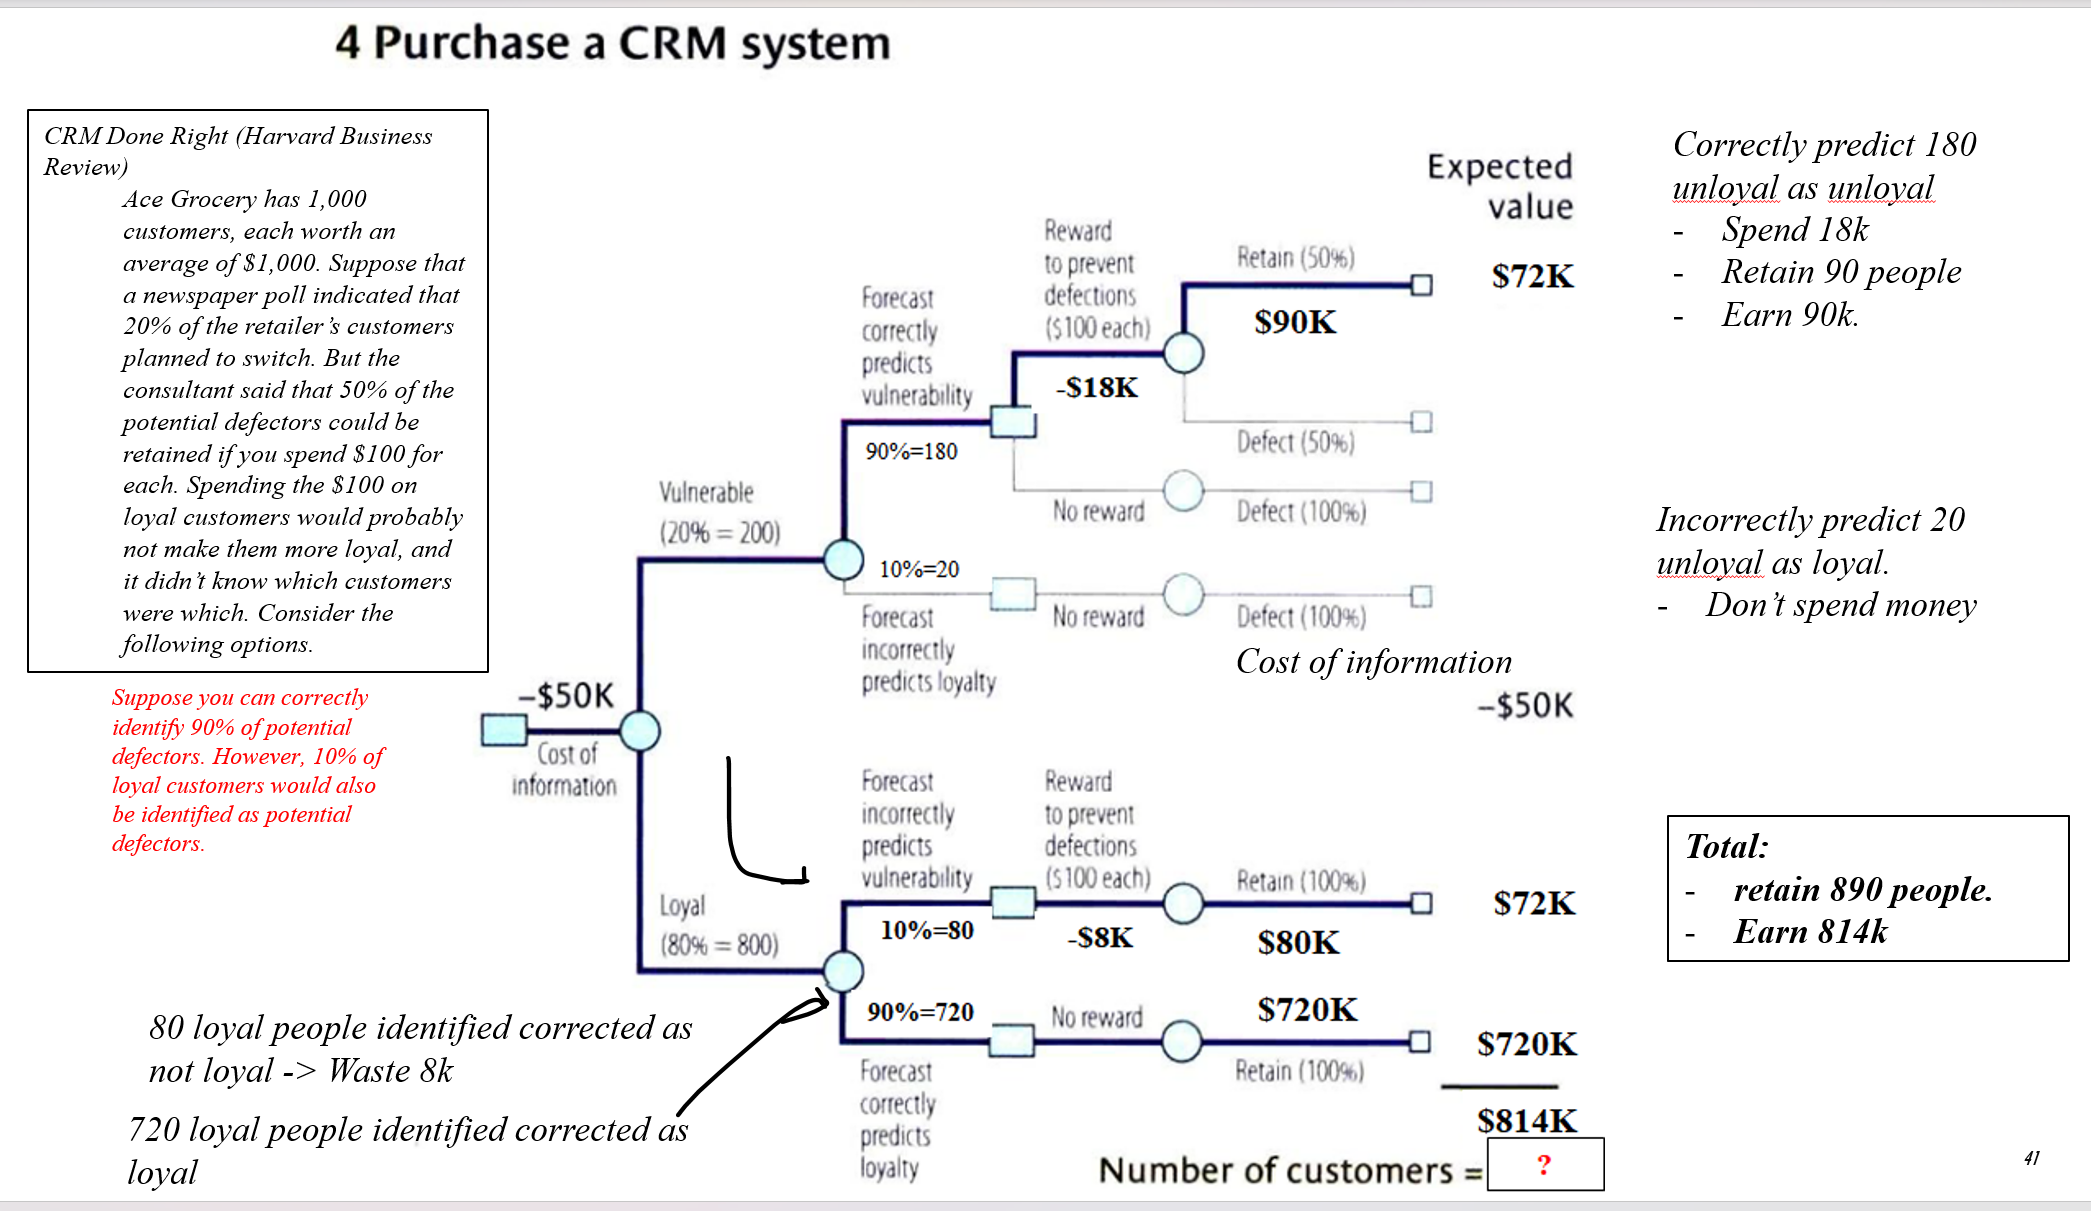
\includegraphics[width=0.80\linewidth]{CRM}}

\vfill\null
\columnbreak

\section{7. Free Riding and Contribution}
\subsection{Private vs. Public Goods}
\begin{itemize}
\item \textbf{Excludable} refers to a good whose ownership or access can be restricted. Usually, private goods are restricted to those who purchase.
\item \textbf{Rivalrous} means that if one person is using it, it diminishes the amount available to another person.
\item \textbf{Private goods} are goods or services that are excludable and rivalrous.
\item \textbf{Public goods} are goods or services that are non-excludable and non-rivalrous.
\end{itemize}
\centerline{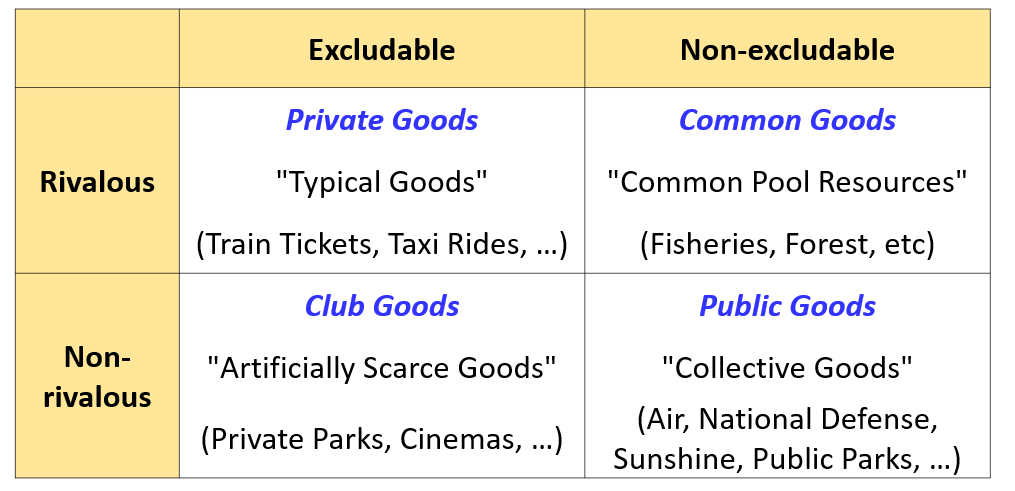
\includegraphics[width =0.5\linewidth]{goods}}
\subsection{Public Goods in the Digital Economy - Undercontribution (Free-Rider Problem)}
\begin{itemize}
\item The existence of many online communities rely on contribution from their users. Examples: Open-source software development communities (e.g., Linux), Wikipedia, Content sharing networks (e.g., Flickr, YouTube), Online Q\&A communities (e.g., Stack Overflow).
\item \textbf{Challenge Faced in Private Provision of Public Goods}: (Contributors are unbalanced, small minority). Many communities rely on “heavy” contributors. This is even more unbalanced in digital economy! Therefore, bigger challenge to how online communities should manage the undercontribution. 
\item \textbf{Participation Inequality in Social Media}: User participation often more or less follows a 90–9–1 rule: (1\% heavy contributors, 9\% Intermittent Contributors and 90\% lurkers, etc.) Such inequities may give you a biased understanding of the community, because you would never hear from the silent majority of lurkers. Customer feedback: customers’ postings may be an unrepresentative sample. Represent only a tiny minority of the people
\item \textbf{“Pareto principle”} (An Italian economist, Vilfredo Pareto, observed in 1906 that a large proportion of the wealth in Italy was owned by a small proportion of the people.) Commonly referred to as the 80-20 principle. For example, businesses often find that a large proportion of sales come from a small proportion of customers. Somewhat consistent with the conventional theory.
\item \textbf{Free Rider Problem} type of market failure that occurs when those who benefit from resources, public goods or services of a communal nature do not pay for them or under-pay. Although there may be a socially optimal outcome, an individual may let others pay
The inability to exclude non-payers is the source of this problem. If non-payers can be excluded by some mechanism, the good may be transformed into a club good.
\item \textbf{Prisoner's Dilemma}: explains. 
\centerline{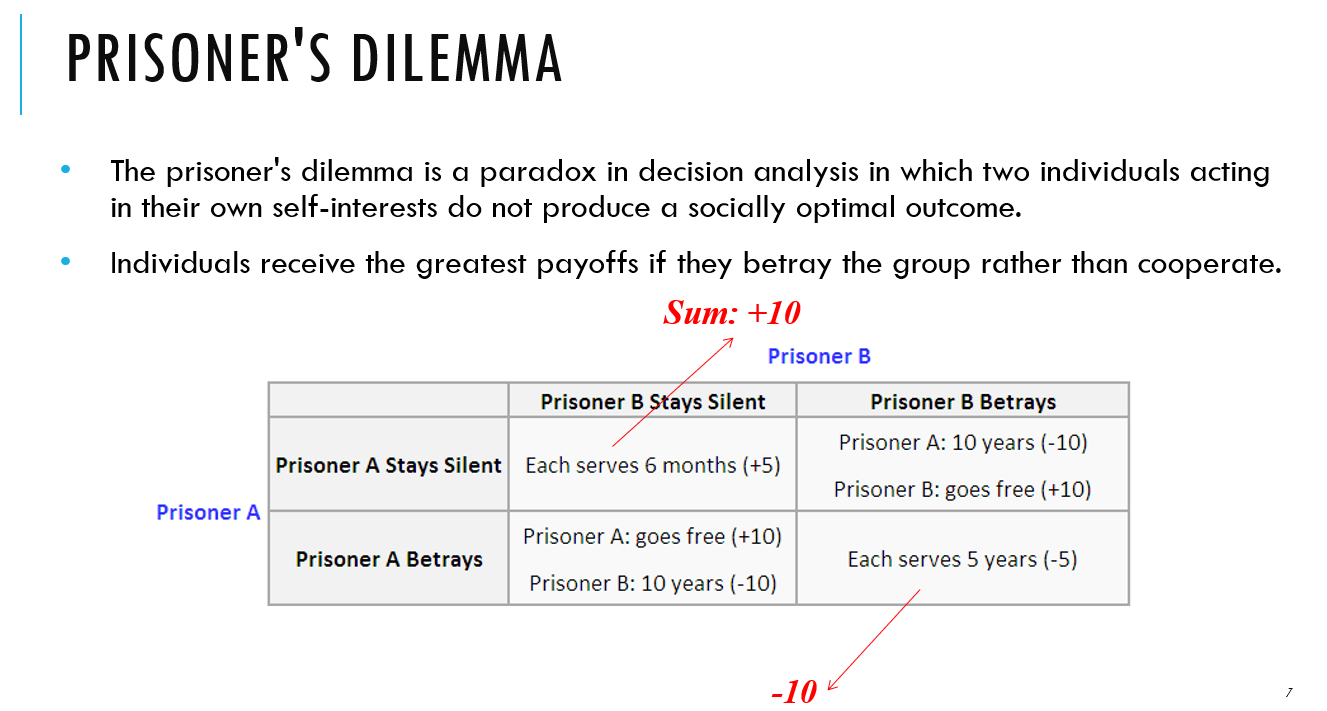
\includegraphics[width = 0.7\linewidth]{prisonerDilemma}}
\end{itemize}
\subsection{Tragedy of the Commons}
\begin{itemize}
\item \textbf{Free Rider Problem, Compounded:}is sometimes compounded by the fact that common goods are characterized by rival consumption, leading to the “Tragedy of the Commons.”
\item \textbf{The Tragedy of the Commons} refers to a situation in which individuals with access to a public resource (also called a common) act in their own interest and, in doing so, ultimately deplete the resource.
\item It initially describes how a common-access sheep-grazing pasture will degrade as each individual herder seeks to improve their own outcome by increasing their own sheep numbers (an individual gain), while the common pasture becomes overgrazed (a collective cost).
\item This theory explains individuals’ tendency to make decisions based on their personal needs, regardless of the negative impact it may have on others. In some cases, an individual’s belief that others won’t act in the best interest of the group can lead them to justify selfish behavior. 
\item \textbf{Examples}: Overfishing, Fast fashion.
\end{itemize}

\subsection{Motivating Participation \& Solutions}
In psychology, motivation may be either intrinsic, if the activity is desired because it is inherently interesting or enjoyable, or extrinsic, if the agent's goal is an external reward distinct from the activity itself.
\begin{itemize}
\item \textbf{Why Contribute?} Pure altruism,Warm-glow giving (emotional reward of giving to others), Fun Reputation/Recognition. (Intrinsic), vs. Reciprocal benefit, Explicit reward (Extrinsic)
\item Make it easier to contribute (lower cost of contribution) \& Reward (but not over-reward) participants: Give contributors some preferential treatment (such as discounts or advance notice of new stuff), or even just put gold stars on their profiles. However, do not overreward, or it will encourage domination of system.
\item \textbf{Social Comparison} In psychology, social comparison theory suggests that people value their own personal and social worth by assessing how they compare to others: Design some series of online performance feedback interventions that aim to motivate the production of user-generated content (UGC).
\item \textbf{Gamification Design}: Gamification is the application of game-design elements and game principles in non-game contexts. Popular and effective strategy in digital economy. Study: Different levels of earned and pursued badges increase the amount of subsequent answering activity.
\end{itemize}

\subsection{Sharing Economy}
An economic model in which goods and resources are shared by individuals and groups in a collaborative way such that physical assets become services. (E.g. Airbnb, Uber, Amazon Turk, CitiBike.)
\begin{itemize}
\item How profitable are bike-sharing systems? They are profitable, to the tune of 1.37 to 1.72 euros of value per 1 euro spent. The authors studied these effects on bike-share programs in 13 European cities. The program investment is presented in orange also included estimates of the positive externalities.
\end{itemize}
\columnbreak

\section{8. Information Asymmetry / Transaction Cost Economics}
\subsection{Information Asymmetry: \& Risk in Economics}
\begin{itemize}
\item \textbf{Information Asymmetry}: Private information that is available to one person but is too costly for others to obtain. Some people have better information than others → Leads to information asymmetry.
\item \textbf{Risk}: Loosely defined as possibility of loss/injury. Despite uncertainty of outcome, decision must still be made, and is based on estimates of expected outcome and attitudes towards risk. Decision maker can be risk averse, neutral or risk taking. Most economic analyses assume risk neutral individuals although most individuals are risk averse.
\item \textbf{Reason for risk}: Uncertainty (Lack of information or asymmetric information). Impact of Risk in economic decision making (buying etc.). We consider Firm and Consumer’s strategies to manage risk.
\end{itemize}
\subsection{Risk Aversion \& Product Quality}
\begin{itemize}
\item \textbf{Willingness to Pay}: Given uncertainty in product quality, consumers have a low willingness to pay (Demand). 2 explored ways to increase WTP: Increase information transparency or give a premium (benefit).
\item \textbf{Ways to Reduce risk and decrease uncertainty for consumers:} Informative advertising (Persuasive techniques but relies more heavily on facts compare to persuasive advertising appealing to consumer emotion), Free Samples or Trials (e.g. Netflix), Money-back guarantees or return policies, Third party quality / reputation certification or review (ISO / Amazon).
\item \textbf{The Economics of Free Trials:} Free tryouts or trials serve the function of providing product quality signals, overcoming the problem of quality uncertainty. Distribution of free (digital) product is similar to advertising in which cost is sunk, but revenue is recovered from future sales.
\end{itemize}
\subsection{Asymmetric Information (Power Imbalance)}
The uncertainty is also related to the well-known phenomenon of information asymmetry between sellers and buyers. Creates an imbalance of power in transactions, which sometimes causes the transactions to be inefficient, causing market failure in the worst case

\subsection{Adverse Selection: Market Failure}
\begin{itemize}
\item \textbf{Adverse selection}: A situation where the more informed party with hidden characteristics (type) use their private information to their own advantage, but to the disadvantage of less informed party.
\item Selection process results in a pool of individuals with undesirable characteristics. Examples: car/medical insurance, loan interest.
\item \textbf{Car Market for Lemon}: In American slang, a lemon is a car that is found to be defective after it has been bought. Suppose buyers cannot distinguish between a high-quality car (a “peach”) and a low-quality one (a “lemon”). Then they are only willing to pay a fixed price for a car that averages the value of a “peach” and “lemon” together. Sellers are better informed about the quality than buyers. Given the fixed price at which buyers will buy, sellers will sell only when they hold “lemons” and they will leave the market when they hold “peaches.” This causes the market to collapse.
\item \textbf{Insurance Market:} Similarly, generally, people who are more at risk and have higher expected losses are more likely to want insurance. This is true in almost all insurance markets (health, car, corporate), and push up the prices for insurances.
\item \textbf{Solutions to Adverse Selection (Signaling, Screening)}: \textbf{Signaling} is where action taken by the informed to reveal private information/hidden characteristics to the uninformed, must not be easily mimicked. E.g. education as signal of work ability, eBay reputation as signal of trading integrity. \\ \textbf{Screening} is where underinformed induces other party to reveal information. Provide a menu of choices in such a way that the choice depends on the private information of other party. Uninformed party then attempts to sort individuals according to their characteristics. Often accomplished through a self selection device. Example: health exam proves health status, second degree price discrimination.
\item \textbf{Quality Uncertainty in Digital Businesses}: Many digital goods are experience goods. (Goods whose quality becomes known only after consumption). Customers may hesitate to consume with a high level of uncertainty (e.g. music, shareware). Quality Uncertainty is compounded by difficulty of ascertaining product attributes over web. Quality uncertainty may be alleviated by Repeat purchases with consumer learning, Seller or buyer reputation build up and Price as a signal for product quality. \textbf{Signaling in Digital Economy}: Foodpanda, Airbnb, Linkedin, Bumble.
\end{itemize}
\subsection{Moral Hazard}
Moral hazard occurs when the ignorant party lacks information about the performance (behaviors) of the agreed-upon transaction or lacks the ability to retaliate for a breach of the agreement.
\begin{itemize}
\item An economic actor has an incentive to increase its exposure to risk because it does not bear the full costs of that risk. For example, when a corporation is insured, it may take on higher risk knowing that its insurance will pay the associated costs.
\end{itemize}
\subsection{Risk Aversion \& Decisions}
\begin{itemize}
\item \textbf{Role of Digital Technologies in tackling these market failures}: Market has become more efficient in that digital technologies enable players to: Reduce uncertainty in a more direct way, offer additional information to reduce information asymmetry and uncertainty, infer better about either party and avoid adverse selection, better observations of behaviors to avoid moral hazard, help enable more effective signaling and screening, employ various digital signals and adopt screening by price discrimination.
\item \textbf{Analytics to infer risk attitudes:} E.g.Use of digital technologies to infer more about consumers (e.g., trustworthiness), Telematics is a method used to collect information about your driving habits (based on your smartphone app). Insurance companies offer some discount for drivers with good habits. Can reduce information asymmetry and thus prevent adverse selection/moral hazard.
\end{itemize}

\vfill\null
\columnbreak

\section{9.  Search Cost \& Transaction Cost}
\subsection{IT Services Market \& Outsourcing }
\begin{itemize}
\item \textbf{IT services market} one of fastest growing segments, encompasses a range of offerings that assist enterprises in implementing, managing and operating a wide variety of systems, software and equipment that are used in modern IT environments. Growth of cloud computing. 
\item \textbf{Gig Economy} A labor market that relies heavily on temporary and part time-positions filled by independent contractors and freelancers rather than full-time permanent employees.
\item \textbf{Freelance Economy}: A labor market consisting of a growing number of short-term contracts.
\end{itemize}
\subsection{Transaction Cost Economics (TCE)}
Explains why companies may break up, may come together.
\begin{itemize}
\item \textbf{Transaction costs (TC)} are expenses incurred when buying or selling a good or service. Transaction costs include the total costs of making a transaction, including the cost of planning, deciding, changing plans, resolving disputes, and after-sales. 
\item \textbf{TCE explains when a firm should expand or not}: If cost of identifying partners, doing business is too high, prefer to do it in house, on my own. If it is low, perhaps should outsource, and focus on my own activities. Also explains when the firm would do better to either break apart or sell off some of its business units. 
\subsubsection{Determinants of TC}
\item Asset specificity, degree to which an asset is specialized for a particular use, which can increase transaction costs by making it difficult to find alternative uses or buyers for the asset.
\item Uncertainty and frequency: The level of uncertainty and frequency of transactions can increase transaction costs by making it difficult to anticipate and coordinate activities between parties.
\item Complexity: The complexity of the transaction can increase transaction costs by making it difficult to communicate and enforce agreements between parties.
\item Bounded rationality: The limited ability of individuals to process and understand all relevant information can increase transaction costs by creating the need for trust, monitoring, and enforcement mechanisms.
\item Opportunism: The potential for one party to take advantage of the other can increase transaction costs by requiring monitoring and enforcement mechanisms to prevent such behavior.
\item \textbf{Implication on Firm Size}: When the external transaction costs are higher than the internal transaction costs, the company will grow. If the internal transaction costs are higher than the external transaction costs the company will be downsized by outsourcing. Context: We have observed an increase in freelancing, outsourcing, and platforms over time, enabled by digital technologies.
\subsubsection{Types of Transaction Costs}
\item Search and information costs (costs associated with looking for relevant information and meeting with agents with whom the transaction will take place.), 
\item Bargaining costs (costs related to coming to an agreement that is agreeable to the parties involved in drawing up a contract.) Bargaining costs can either be very cheap, such as buying a newspaper, or can be very expensive, such as trading a soccer player from one team to another.
\item Policing and enforcement costs: associated with making sure that the parties in the contract keep their word and do not default on the terms of the contract. In the real world, people often deviate from the contract, and thus, enforcement costs are incurred while governing contracts. Lawyer fees are an example of such a cost.
\end{itemize}
\subsection{Digital Revolution and impact on types of TCE}
New digital technologies are likely to reduce transaction costs comparatively to traditional forms of contracting.
\begin{itemize}
\item \textbf{Search and information costs:} Big data and analytics to reduce information asymmetry
\item \textbf{Bargaining costs: Scale of collaboration} (Ex: Big data and AI, blockchain) Speed of collaboration (Ex: 5G/6G network)
\item \textbf{Policing and enforcement costs:} Better monitoring (Ex: Big Data, AI, IoT, …)
\item \textbf{Networks Invert the Firm} Firms tap ideas they haven’t yet imagined from third parties they don’t even know: Inversion extends outsourcing.
\item \textbf{Harnessing Spillovers}: Utilizing big data analytics, network effect. Positive spillover effects help platforms rapidly increase the volume of interactions. E.g. Book purchase reccomendations. Dynamic exploits the fact that network effects are often strongest among interactions of the same type.
\end{itemize}
IT makes building and scaling up platforms vastly simpler and cheaper, strengthens network effects, and enhances the ability to use big data to increase platform’s value .
\subsection{Platforms in TCE (Impact on Traditional Pipeline Businesses)}
\begin{itemize}
\item \textbf{Traditional economies:} Businesses that have dominated industry for decades. Pipeline businesses create value by controlling a linear series of activities—the classic value-chain model. The economies of scale is the key in this economy (e.g., Walmart).
\item Digital technologies enabled new forms of organizations and a prosperity of platform businesses. The network effect is the key for the success of platform economy (e.g., Apple).
\end{itemize}

\subsection{Platforms vs. Pipelines}
\begin{itemize}
\item \textbf{Platforms require new ways of thinking instead of five- forces model}: “Platform” businesses that bring together consumers and producers, as Uber, Alibaba, and Airbnb require a different approach to strategy. The critical asset of a platform is external—the community of members. 
\item Shifts from controlling resources to orchestrating them, firms win by facilitating more external interactions and creating “network effects” that increase the value provided to all participants.
\item Competition can emerge from seemingly unrelated industries and even from within the platform itself.
\item When a platform enters the marketplace of a pure pipeline business, the platform nearly always wins. 
\end{itemize}
\textbf{Move from pipeline to platform involves three key shifts}
\begin{itemize}
\item \textbf{1. From resource control to resource orchestration}:With platforms, the assets that are hard to copy are the community and the resources its members own and contribute, be they rooms or cars or ideas and information. In other words, the network of producers and consumers is the chief asset.
\item \textbf{2. From internal optimization to external interaction}: Platforms create value by facilitating interactions between external producers and consumers. Because of this external orientation, they often shed even variable costs of production. 
\item \textbf{3. From a focus on customer value to a focus on ecosystem value.}: Pipelines seek to maximize the lifetime value of individual customers of products and services, who, in effect, sit at the end of a linear process. By contrast, platforms seek to maximize the total value of an expanding ecosystem in a circular, iterative, feedback-driven process. Sometimes that requires subsidizing one type of consumer in order to attract another type.
\item \textbf{Platform Players}
\centerline{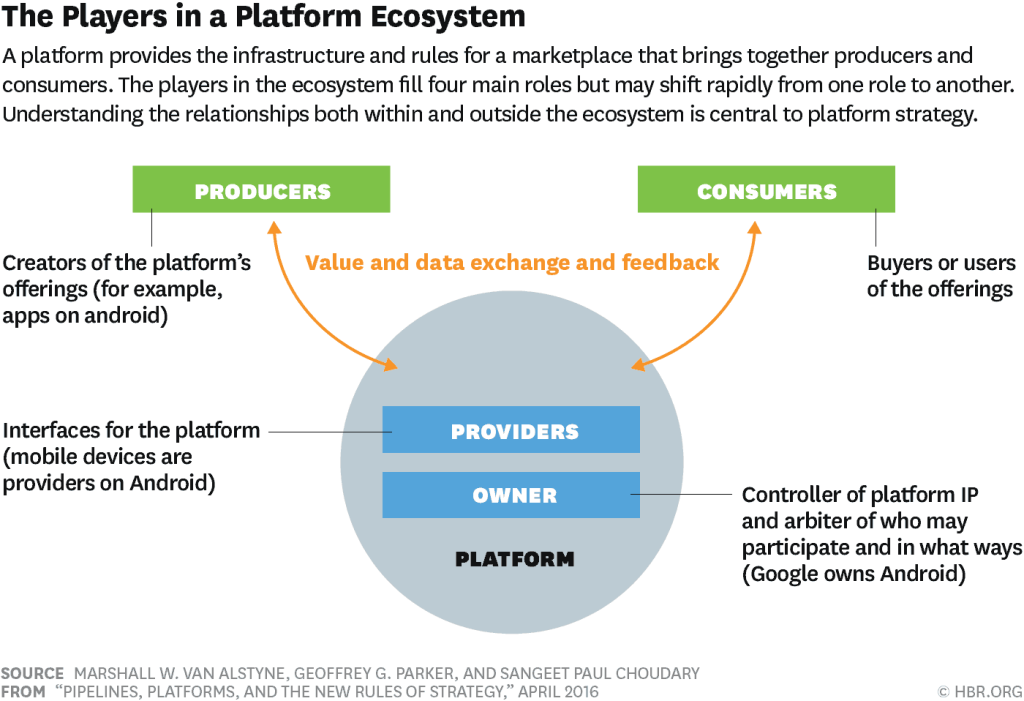
\includegraphics[width = 0.8\linewidth]{platformPlayers}}
\item Platforms must understand the financial value of their communities and their network effects. While pure platforms naturally launch with an external orientation, traditional pipeline firms must develop new core competencies—and a new mindset—to design, govern, and nimbly expand platforms on top of their existing businesses.
\item \textbf{The failure to transition} to a new approach explains the precarious situation of traditional businesses (hotels, health care providers) For pipeline firms, there is need to learn the new rules of strategy or risk losing.
\end{itemize}


\subsection{“Long Tail Phenomenon”}
\begin{itemize}
\item “Consumers’ preferences in IT-enabled markets have greater depth than in typical brick-and-mortal stores”. Sales still present (and substantial) for ‘not so popular’ variety products.
\centerline{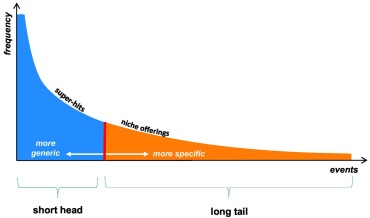
\includegraphics[width = 0.7\linewidth]{longtail}}
\item The online marketplace has enabled consumers in many industries to locate, evaluate and purchase a far wider variety of products than they can via traditional brick-and-mortar channels.
\end{itemize}

\subsection{Search Cost }
\begin{itemize}
\item \textbf{Search cost} is the time, energy, and money that buyers and sellers in a market expend in trying to find one another in order to engage in transactions.
\item - Search costs include the opportunity cost of the time and effort spent on searching plus any explicit costs of money or scarce resources expended in searching. The internet and digital technologies have greatly reduced consumers’ search costs
\item Internet provides marketers with new ways of identifying and communicating with customers: \textbf{Long tail marketing:} ability to reach a large audience inexpensively/ \textbf{Behavioral targeting:} tracking online behavior of individuals on thousands of Web sites
\item By greatly lowering search costs, information technology in general and Internet markets in particular could substantially increase the collective share of hard-to-find products, thereby creating a longer tail in the distribution of sales.
\item \textbf{What if search costs become 0?} There may be no price dispersion (i.e., different sellers offer different prices for the same good in a given market) for standardized products! ervice component of product would become more important for differentiation. Consumers can buy a product that would best meet their individual needs and taste. Retailers will have to meet consumers’ needs by selling more diverse and/or customized products
\item \textbf{Search Cost across Channels}: The Internet channel’s Lorenz curve lies above the catalog channel’s Lorenz curve, implying that the Internet channel exhibits a less concentrated distribution of product sales than the catalog channel. 
\centerline{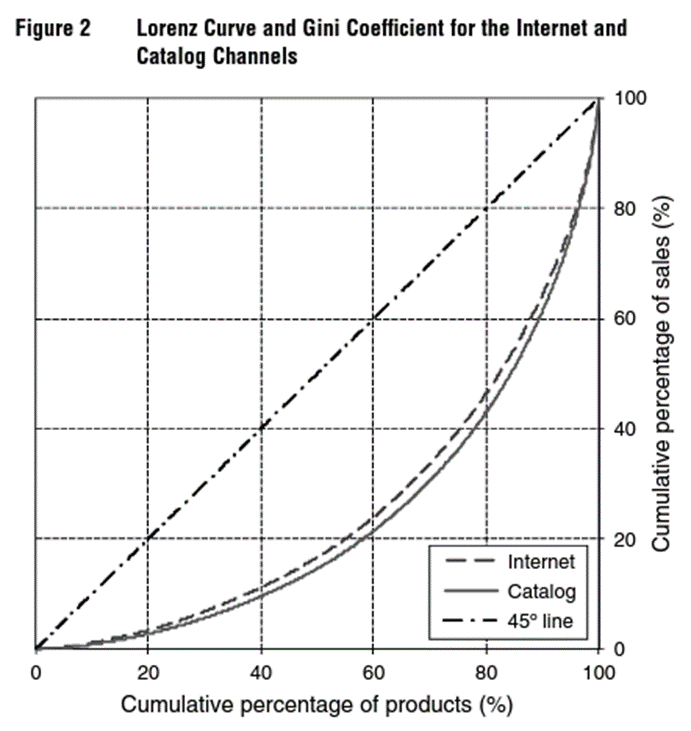
\includegraphics[width = 0.3\linewidth]{searchGini}}
\item Correspondingly, the Gini coefficient for the Internet channel (0.49) is lower than that for the catalog channel (0.53). Importance of meeting diverse needs of consumers from different channels that involve different levels of search cost.
\end{itemize}


\vfill\null
\columnbreak

\section{10: Behavioral Economics}
\begin{itemize}
\item \textbf{Behavioral Economics} combines elements of economics and psychology to understand how and why people behave the way they do in the real world. Differs from neoclassical economics, which assumes that most people have well-defined preferences and make well-informed, self-interested decisions based on those preferences. 
\item \textbf{[Grounded in] Empirical observations of human behavior}, which have demonstrated that people do not always make what neoclassical economists consider the “rational” or “optimal” decision, even if they have the information and the tools available to do so. (People are sometimes irrational)
\end{itemize}
\subsection{Nudging}
\begin{itemize}
\item \textbf{Nudge}: Thaler and Sunstein (2008, p. 6), is any aspect of the choice architecture that alters people's behavior in a predictable way without forbidding any options or significantly changing their economic incentives.
\item Examples: Placing healthier food choices at eye level or near cash register in schools, compared to banning junk food. Thaler: Changing test scores to be out of 137 instead of 100. Study that yielded fuel savings in flights.
\end{itemize}
\subsection{Loss Aversion}
\begin{itemize}
\item In general, if dealing with loss aversion, people are more willing to take risk (to avoid loss). With “prospect theory,” Tversky and Kahneman demonstrated that framing and loss aversion influence the choices people make. 
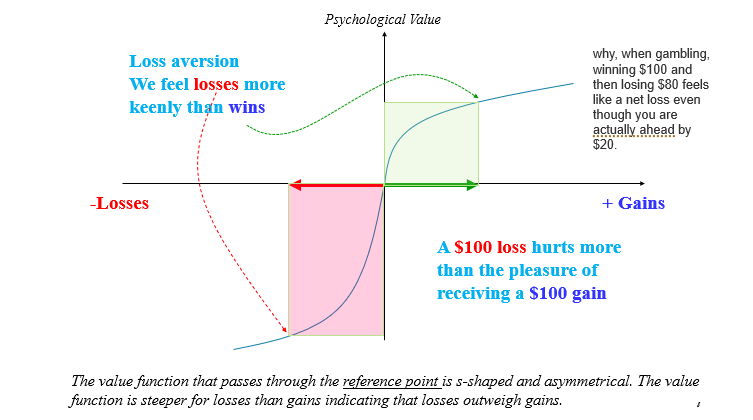
\includegraphics[width =\linewidth]{lossAversion}
\end{itemize}
\subsection{Confirmation Bias}
\begin{itemize}
\item Refers to people's tendency to process information by looking for, or interpreting, information that is consistent with their existing beliefs.This biased approach to decision making is largely unintentional, and it results in a person ignoring information that is inconsistent with their beliefs.
\item In social media, confirmation bias is amplified by the use of filter bubbles, or "algorithmic editing", which display to individuals only information they are likely to agree with, while excluding opposing views.\item A filter bubble is a state of intellectual isolation that can result from personalized searches, where a website algorithm selectively curates what information a user would like to see based on information about the user, such as location, past click-behavior, and search history.
\end{itemize}
\subsection{Sunk Cost Fallacy}
\begin{itemize}
\item \textbf{Sunk Cost}: Refers to money that has already been spent and cannot be recovered.
\item The sunk cost fallacy refers to a greater tendency to continue an endeavor once an investment in money, effort, or time has been made. This is like "throwing good money after bad“.
\item Even though economists argue that sunk costs are not at all relevant to future rational decision-making, people in everyday life often take previous expenditures in situations, such as repairing a car and gambling loss into their future decisions regarding those properties.
\end{itemize}
\subsection{Digital Nudging}
\begin{itemize}
\item A subtle form of using design, information and interaction elements to guide user behavior in digital environments, without restricting the individual's freedom of choice.
\item The use of digital nudges has become prevalent and is widely adopted in various domains. With digital technologies, it is much easier to implement such “nudges” and influence user behaviors (recall the “zero marginal cost” in digital economy) In addition, we spent more and more time with digital technologies.
\item Re-analysis of meta-analysis reveals no evidence for nudging once accounting for publication bias: A 2022 meta-analysis that nudging was an effective tool for behavior modification. However, the authors also found significant publication bias toward positive results in the literature, with a sensitivity analysis revealing a miniscule effect size in the case of severe publication bias.
\item In reality, designing appropriate nudges that work consistently and reliability is very challenging.
\end{itemize}
\subsection{Field Experiment (AB Test)}
\begin{itemize}
\item A/B testing, also known as split testing, refers to a randomized experimentation process wherein two or more versions of a variable (web page, page element, etc.) are shown to different segments of website visitors at the same time to determine which version leaves the maximum impact and drives business metrics.
\item \textbf{p-Hacking}: defined as “try[ing] out several statistical analyses and/or data eligibility specifications and then selectively report[ing] those that produce significant results. They may stop their experiments based on the p-value of the treatment effect. Study found false discovery rate (FDR) ranges between 28\% and 37\% for tests conducted at 10\% significance level (less robust).
\end{itemize}

\vfill\null
\columnbreak


\section{11: Economic Impacts of AI}
\subsection{Artificial Intelligence}
\begin{itemize}
\item Broadly speaking, AI refers to the ability of a digital computer or computer-controlled robot to perform tasks commonly associated with intelligent beings.
\item Characterizing AI precisely is also difficult because the definition tends to change depending on the specific context of research and application. AI is widely used to analyze big data, identify patterns, and predict outcomes
\item \textbf{Turing Test} to define AI: If a computer can talk like a human and cannot be told apart, then the computer can think like a human. ChatGPT is known to have passed the Turing test.
\end{itemize}
\subsection{Labor Substitution by AI}
\begin{itemize}
\item Who will be replaced? Who will do a better job does not necessarily mean the actual or immediate replacement. That is, it is not matter of efficiency or technology. Additionally, income or social status does not necessarily mean a lower chance of replacement either.
\item \textbf{Investment and Employment}: Impact on employment not obvious yet. Data from robots imported by Canadian firms by the Canadian Border Services Agency (CBSA) from 1996 to 2017, found that: Robots may directly reduce need to monitor workers when robots reduce human errors in production process. Although the total number of nonmanagerial employees increases with robot adoption, robot investments predict decreases in employment of middle-skilled workers and increases in employment of low- and high-skilled labor
\item “From Agriculture to Art — the A.I. Wave Sweeps In,” NY Times, (2018): Artificial intelligence is a technology of low-cost prediction and discovery. It exploits the new resource of the digital age —vast amounts of data —to identify patterns and make predictions. Much of what A.I. does today can be thought of as a prediction.
\end{itemize}
\subsection{Economic Impact at Different Levels}
\begin{itemize}
\item In general, the impact of digital technologies we have discussed will be amplified. However, we will have to deal with many new issues. It is very difficult to predict what is going to happen at this point.
\item \textbf{Country}: Digital divide will be reinforced, The gap between leading countries and developing countries will be widened. Retraining will become a critical issue. New business models also possible.
\item \textbf{Company}: Performance gap will be widened between front-runners and non-adopters, Use AI for labor augmentation or substitution of production factors
\item \textbf{Individual / Workers}: More jobs will be replaced or augmented with AI.
\end{itemize}
\subsection{Adoption of AI by Companies \& Issues}
\begin{itemize}
\item On top of technological issues, companies need to address more issues to adopt AI in businesses: Black box problem, Consumer reaction, Regulation and Ethical issues.
\item \textbf{Black Box Problem}: (Lack of explanability) As models become more sophisticated they begin to evolve from simple linear models to non-linear combinations, occasionally of other more complicated models. This is known as the “Black Box Problem” in machine learning. This significantly limits the applicability of AI models especially when the failure in systems leads to a serious problem (e.g., threatening human lives)
\item \textbf{Consumer Reactions}: Consumers may react either positively or negatively to Ais depending on the different contexts. Anthropomorphism is one of the important elements to be considered for robots and AI. It is generally described as “the attribution of human-like qualities to nonhuman entities such as machines, animals, and other objects: Uncanny Valley: 1970s, Professor Masahiro Mori, observation that as robots appear more humanlike, they become more appealing - but only up to a certain point. Upon reaching the uncanny valley, our affinity descends into a feeling of strangeness, unease, and freakiness. Justifies people’s negative reaction to certain lifelike robots.
\item Results suggest that undisclosed chatbots are as effective as proficient workers and four times more than inexperienced in engendering customer purchases. However, disclosure of bot identity before the convo reduces purchase rates by more than 79.7\%.
\end{itemize}

\vfill\null
\columnbreak


\section{12: Risks and Regulation of AI}










\end{multicols*}
\end{document}
